
\begin{figure}[H]
\begin{center}
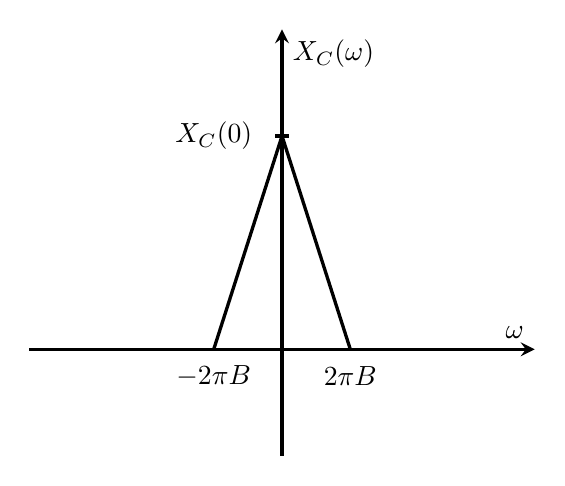
\begin{tikzpicture} 
\tikzset{every pin edge/.style={scale=0.00001}    }
\begin{axis}[very thick,
                     samples = 100,
                     ytick={-2,2},
                     xlabel = {$\omega$},
                     ylabel = {$X_C(\omega)$},
                     xmin = -3.7,
                     xmax = 3.7,
                     ymin = -0.5,
                     ymax = 1.5,
                     width=8cm,
                     height=7cm,
                     axis x line = middle,
                     axis y line = middle,
                     ticks = none]
                     
            \addplot[mark=none] coordinates {(-1,0) (0,1)};
            \addplot[mark=none] coordinates {(0,1) (1,0)};
            \addplot[mark=none] coordinates {(-0.1,1) (0.1,1)};
            \node at (axis cs:-1,1){$X_C(0)$};
            \node at (axis cs:1,-0.125){$2\pi B$};
            \node at (axis cs:-1,-0.125){$-2\pi B$};
            
        \end{axis}
\end{tikzpicture}
\end{center}
\caption{Espectro de magnitude de $X_C(\omega)$. Sendo $B$ dado em Hz. Fonte: própria.}
\label{graph:1} 
\end{figure}